\section{Supervised learning에서 Training의 원리}
    Supervised Learning은 Training Data와 그에 대한 정답에 해당하는 Label을 활용하여 모델을 학습하는 Machine Learning 방법론이다. Training Data와 Label로부터 모델을 학습시켜 새로운 입력 데이터에 대한 Label을 예측한다. \\
    \vspace{-4mm}
    \begin{figure}[!h]\centering
	    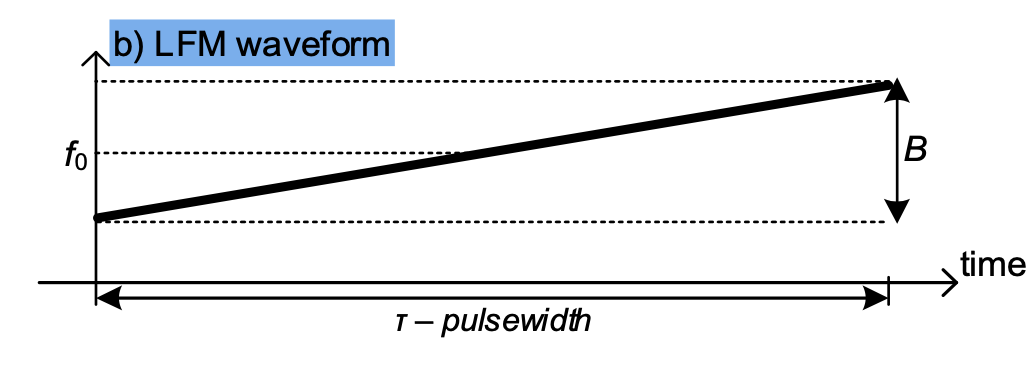
\includegraphics[width=.65\textwidth]{image/week04/1-1.png}
	    \caption{\small Supervised Learning Algorithm}
	    \vspace{-10pt}
    \end{figure}
    
    \subsection{Supervised Learning의 종류}
    Supervised Learning Algorithm은 크게 Classification 와 Regression으로 나뉜다. 
    \vspace{-4mm}
    \begin{figure}[!h]\centering
	    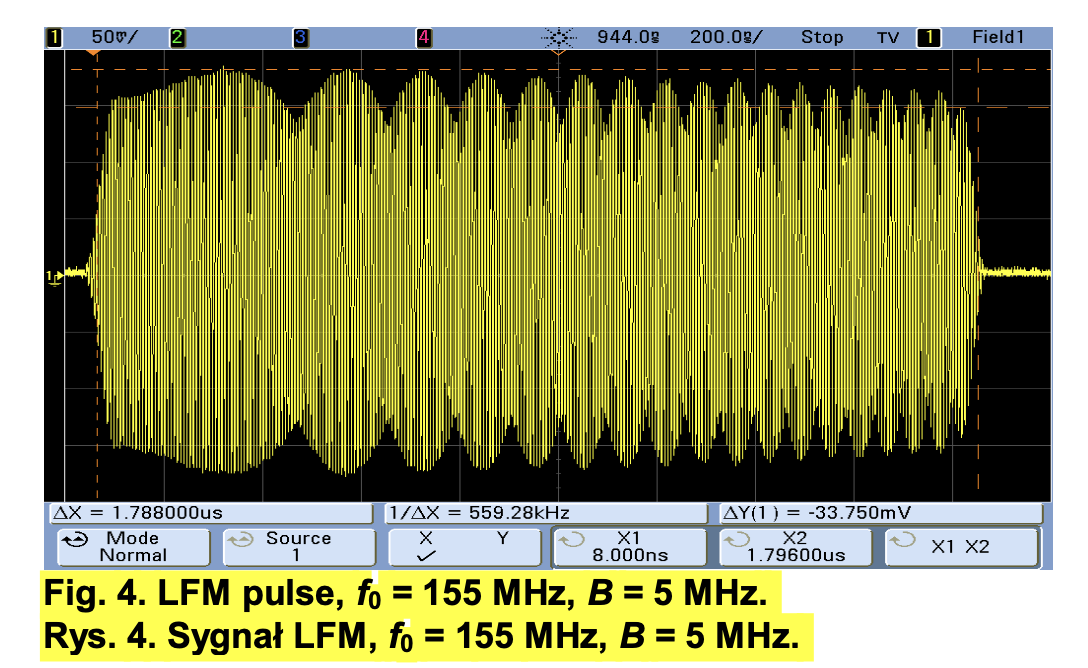
\includegraphics[width=.65\textwidth]{image/week04/1-2.png}
	    \caption{\small Classification and Regression}
	    \vspace{-10pt}
    \end{figure}
    
    \subsubsection*{Classification}
    Classification은 입력 데이터에 대응하는 label이 두 가지 혹은 여러 가지로 서로 구분되는 범주형 데이터인 경우 사용한다. 예를 들어 입력 데이터로 메일과 메일이 스팸 메일이다, 아니다를 label로 주고 Classification 학습을 한다면 새로운 메일에 대하여 스팸메일 인지 아닌지 분류를 할 수 있다.  Classification에는 다음과 같은 알고리즘들이 있다 : 
    \begin{enumerate}
        \item 선형 펀별 분석
        \item KNN (k- Nearest Neighbor)
        \item Tree 
        \item Neural Network
        \item Support Vector Machine 
    \end{enumerate}
    
    \subsubsection*{Regression}
    Regression은 입력 데이터에 대응하는 label이 어떠한 범위 내에서 자유롭게 수치 형태로 존재하는 연속형 데이터인 경우 사용한다. 예를 들어 아파트 가격을 예측하는 알고리즘을 Regression으로 학습할 수 있을 것이다. 아파트의 위치, 채광, 대중교통 및 지역 시설과의 근접성, 해당 지역의 사회경제적 인구 통계, 현재 시장 상황 등의 변수를 입력 데이터로, 아파트 가격을 label로 사용할 수 있다.